\chapter{Résultats et perspectives}

\section{Résultats}

\begin{itemize}
  \item surface
\end{itemize}

Nous sommes donc capables, étant donné un complexe stocké dans un fichier \textit{.pdb},
d'afficher ce complexe (voir figure \ref{fig::complexe}) et de visualiser la surface
de contact dans Meshlab (voir figure \ref{fig::affichage_final}).

\begin{figure}[ht]
\centering
  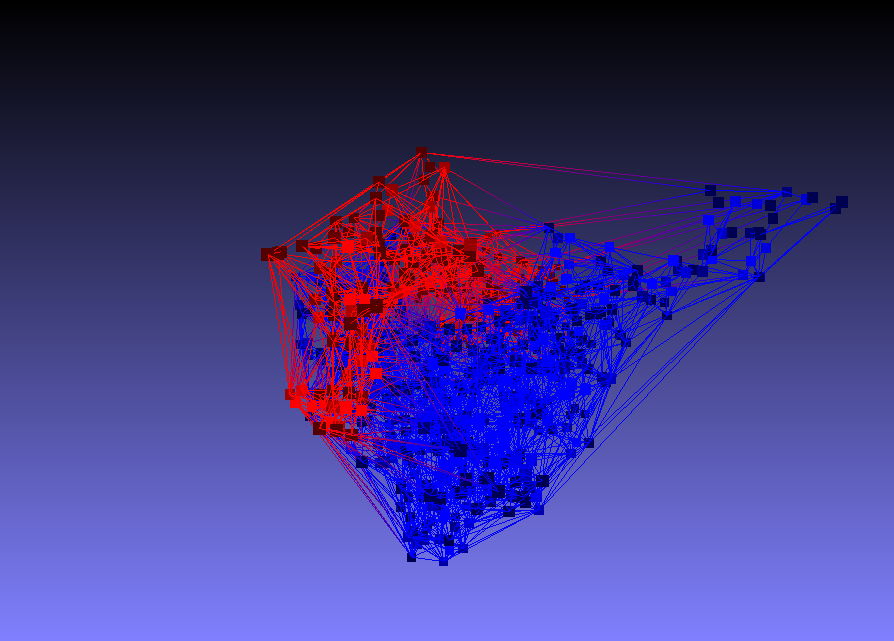
\includegraphics[width=0.8\textwidth]{figures/final_no_surf.png}
  \caption{Complexe}
  \label{fig::complexe}
\end{figure}

\begin{figure}[ht]
\centering
  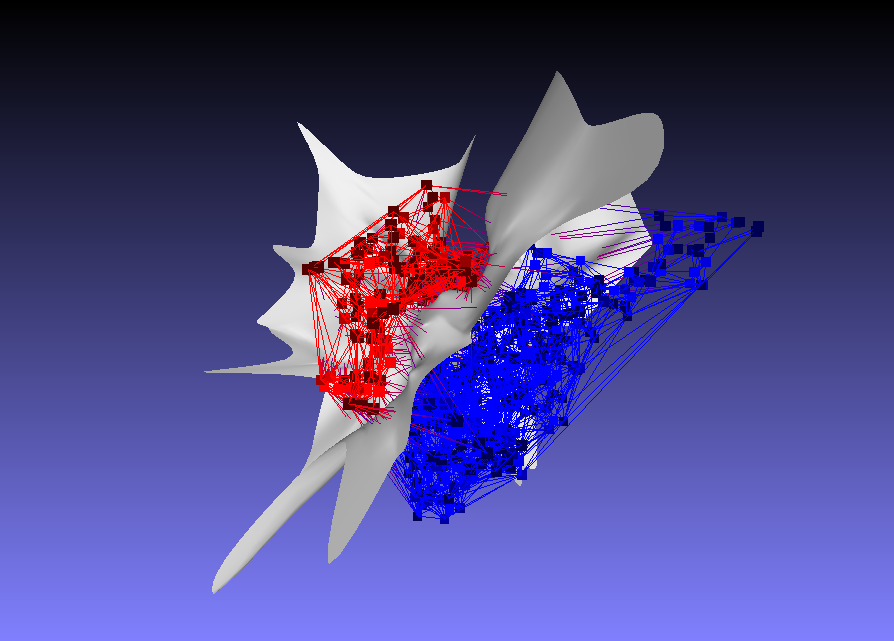
\includegraphics[width=0.8\textwidth]{figures/final_with_surf.png}
  \caption{Affichage de l'interface entre deux protéines}
  \label{fig::affichage_final}
\end{figure}

La méthode d'indexation permet de connaître à tout moment les particularités de chaque
atome et de lier ces informations à la surface. Les deux atomes formant une arête
de l'interface correspondent à un morceau de la surface.



\section{Perspectives}
\begin{itemize}
  \item Fonctionnalités
\end{itemize}

La méthode d'affichage utilisée (indexation des points et affichage par triangles)
peut permettre de passer facilement en OpenGL.
